
\section{Dynamical Systems}\label{sec:dyn-systems}
Consider our go-to differential equation:
$$ X' = AX $$
where $A$ is some fixed matrix. We know the general solution is given by $$ X(t) = e^{tA}v $$ where $v$ is determined by the initial conditions. There are two ways we may wish to study this equation. We could fix $v$ and consider how the equation behaves as we vary $t$. This gives us exactly the trajectory or orbit of a solution.

On the other hand, we could fix $t$ and consider what happens as we vary $v$. Such a map is often denoted $\Phi_t$ is known as the \textit{flow} of the system (this function maps some initial point to where it would be sent by the solution at time $t$). What we get then is a map from $v$ to $e^{tA}v$, which in this case is simply a linear isomorphism on $\R^n$. We in fact have a family of isomorphisms $\{e^{tA}\}_{t \in \R}$ that satisfy the following property: $e^{0A} = \text{Id}$ and $e^{(t + s)A} = e^{tA} e^{sA}$. A family of bijective maps $\{\phi_t\}_{t \in \R}$ on $\R^n$ that satisfies these properties (i.e. $\phi_0 = \text{Id}$ and $\phi_{s + t} = \phi_s \circ \phi_t$) is called a dynamical system. In different areas of math, we make different assumptions on the properties that the $\phi_t$ must satisfy. For our purposes, we assume them all to be smooth. In principle we index simply over the positive reals or the natural numbers (which would be like looking at discrete time). If we were feeling particularly adventurous, we could replace $\R^n$ with a manifold instead. But for now, we leave things as they are.

It is perhaps useful to consider why the `semigroup property' of dynamical systems (i.e. that $\phi_{s + t} = \phi(s) \circ \phi(t)$ is important. The claim is that with this property, by only looking at the initial conditions, we can in fact study all solutions. This is because the semigroup property allows us to `stitch together' solutions in a certain sense. Suppose we have a solution that begins at $x$ and passes through $y_1$ in time $t$. Suppose we have another solution that starts at $y_1$ and reaches $y_2$ in time $s$. Then one would hope that the original solution that began at $x$ also reaches $y_2$, but at time $s + t$ (and in fact hopefully the path from $x$ to $y_2$ would be given by combining/stiching together the two solutions in the obvious manner, should this be possible). This is exactly the property characterised by the semigroup property.

\begin{figure}[h]
    \centering
    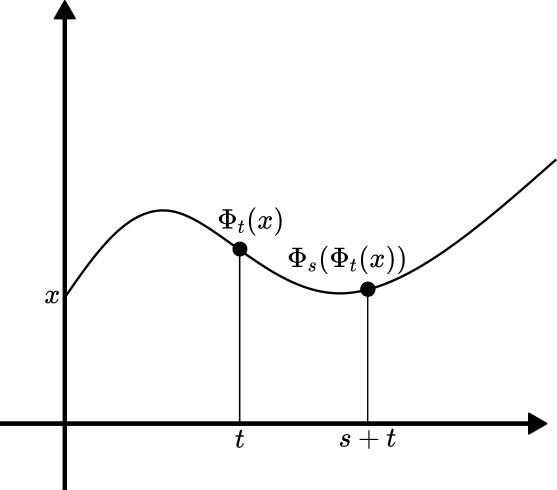
\includegraphics[scale=0.7]{Images/flow_semigroup.png}
    \caption{The semigroup property of flow. We evolve for time $s$ from $\Phi_t(x)$. This corresponds exactly with evolving for time $s + t$ from $x$.}
    \label{fig:flow-semigroup-prop}
\end{figure}


\section{Existence and Uniqueness of solutions}
The existence and uniqueness of solutions is of course a key point with differential equations. We have already said that most differential equations can't be solved explicitly. Part of the problem is that there may be no analytic solution. However, the situation may be even more dire than that: there may genuinely be no solution. Suppose we are given that
\begin{align*}
    x' = \begin{cases}
    -1, & x \geq 0\\
    1, & \text{otherwise}
    \end{cases}
\end{align*}
Consider the situation at $x = 0$. At this point, the point `wants' to decrease due to it negative gradient. However as soon as it does so, the derivative becomes positive causing it to move up. Hence why the above differential equation has no solutions. We can argue more precisely using a statement in analysis which tells us that the derivative of a function can never have a jump discontinuity (roughly speaking a jump discontinuity means that the left and right hand limits of a function differ, however the derivative of a function at a point is a limit so we know if it exists, the left and right hand limits are the same). Hence we know that if a solution to $x' = f(x)$ is to exist then $f$ must at the very least be continuous.

Sometimes solutions may exist but need not be unique. Suppose we have
$$x' = 3x^{2/3}$$
with initial condition $x_0 = 0$. Then $x(t) = 0$ and $x(t) = t^3$ are both solutions that satisfy this initial value problem. The problem here is that $f$ is continuous but not smooth (or even differentiable everywhere). In fact what we will see is that given $x' = f(x)$, we are guaranteed to have unique solutions to the ODE, if $f$ is continuously differentiable. However, it is hard to ensure that we have a solution that is defined everywhere as is illustrated by equation
$$x' = x^2$$
whose general solution is given by
$$x(t) = \frac{x_0}{1 - x_0 t}$$
We see that this is not defined at $t = x_0^{-1}$. This leads us to the local uniqueness and existence theorem.

\begin{theorem}[Local Existence and Uniqueness]
    Suppose we are considering the ordinary differential equation $X' = F(X)$ where $F: \R^n \to \R^n$ is continuously differentiable. Then for all $a \in \R^n$ there exists an interval $I = (\alpha, \beta)$ containing the origin such that $X' = F(X)$ has a unique solution $X: I \to \R^n$ satisfying $X(0) = a$.
\end{theorem}

Although we will get on to proving this theorem soon enough, let us consider some of its consequences. For example, if we have two solutions where the corresponding intervals intersect, is it the case that the solutions agree on the intersection? The answer is yes. This follows from uniqueness of the solutions: take a point in the intersection and use this to define our initial condition. We know that both solutions solve the differential equation, therefore must be equal (on the intersection). This suggests that we can `patch' together local solutions (as discussed previously) to get solutions defined on a larger interval. By pasting together all the local solutions, we can get a maximal interval of existence (to be precise, the interval can be found by taking union of the intervals guaranteed by the above theorem as we range over all the point in $\R^n$).

\subsection{Preliminary Theory}
There are several results we need before we can prove the local existence and uniqueness theorem. On account of the author being too small brain, we largely only include the definitions and statements of the theorems we need and omit the proofs.

Because we will refer to it many times, we also include the definition of uniform continuity and uniform convergence.
\begin{definition}[Uniform Continuity]
A function $f: E \to \R^m$ is said to be uniformly continuous if for every $\epsilon > 0$ we can find a $\delta > 0$ such that given $x, y \in E$ satisfying $|x - y| < \delta$, we have $|f(x) - f(y)| < \epsilon$ (in particular the choice of $\delta$ is independent of $x$ and $y$).
\end{definition}
\begin{definition}
A sequence of functions $\{f_n: E \to \R^m\}$ is said to converge uniformly to a function $f: E \to \R^m$ if for every $\epsilon > 0$ there exists some $N \in \N$ such that
$$ \sup_{x \in E} |f_n(x) - f(x)| < \epsilon $$
for every $n \geq N$.
\end{definition}
Recall that if a sequence of continuous functions converges uniformly then the function they converge to is also continuous.

\begin{definition}[Uniformly Bounded]
Let $\{f_\alpha\}$ be a family of functions where each $f_\alpha$ is a map from $E \subset \R^n$ to $\R^m$. Suppose there exists some $M$ such that $|f_\alpha(x)| < M$ for all $x \in E$ and all $\alpha$. Then we say that the $\{f_\alpha\}$ are uniformly bounded.
\end{definition}
\begin{definition}[Equicontinuous]
Let $\{f_\alpha\}$ be a family of functions where each $f_\alpha$ is a map from $E \subset \R^n$ to $\R^m$. The $\{f_\alpha\}$ are said to be equicontinuous if for every $\epsilon > 0$ we can find some $\delta > 0$ such that for all $x, y \in E$ and for all $f_\alpha$, if we have $|x - y| < \delta$ then $|f_\alpha(x) - f_\alpha(y)| < \epsilon$ (in particular the choice of $\delta$ is independent of $x, y$ and $\alpha$).
\end{definition}

\begin{example}
The family of functions $f_{\alpha}(x) = \alpha x$ for $\alpha \in \R$ is not equicontinuous. If we instead restrict $\alpha$ to be in $[3, 5]$ (or any bounded interval) then the family of functions is equicontinuous.
\end{example}
\begin{example}
The family of functions $f_n(x) = x^n$ defined on the unit interval $[0, 1]$ is not equicontinuous.
\end{example}
\begin{example}
A family of Lipschitz functions which share the same Lipschitz constant is equicontinuous.
\end{example}
\begin{example}
Any finite family of uniformly continuous functions is equicontinuous.
\end{example}

We can define the sup norm on a function space where if $f: E \to \R^m$ then
$$ \norm{f}_\infty = \sup_{x \in E} |f(x)| $$
The space of continuous functions on $[0, 1]$ is often denoted $C([0, 1])$. We claim that that $C([0, 1])$ equipped with $\norm{\cdot}_{\infty}$ is a complete metric space. This is exactly the statement that the uniform convergence of a sequence of continuous functions is also continuous.

\begin{theorem}
    Suppose $f_n: E \to \R^n$  is a sequence of continuous maps. If $E$ is compact and and the $\{f_n\}$ converge uniformly, then the $\{f_n\}$ are uniformly bounded and equicontinuous.
\end{theorem}
\begin{proof}
Let $f$ denote the limit of the $f_n$. We first show uniform boundedness. Since each $f_n$ is continuous and $E$ is compact, we know there exists some constant $M_n$ such that $|f_n(x)| \leq M_n$ (indeed we can take $M_n$ to be $\norm{f_n}_{\infty}$). Since $f$ is also continuous, it is also going to be bounded by some $M_0$.

The idea is that eventually all the $f_n$ are going to be quite close to $f$ therefore we should able to bound (bind?) all but finitely many of them with $M_0$ (or something close to it at least). Then we are only left with finitely many bounds so the maximum of all of these should bound all the $f_n$. Let us formalise this.

Let $N$ be such that for all $n \geq N$ we have that $\norm{f - f_n}_{\infty} < 1$ (this is equivalent to saying that $|f(x) - f_n(x)| < 1$ for all $x \in E$). The existence of such an $N$ is guaranteed by uniform continuity. Let $M = \max\{M_0 + 1, M_1, \dots, M_{N}\}$. We claim that $M$ is a bound for all the $f_n$. Clearly this holds true for $n \leq N$. Suppose $n > N$. Then
$$ \norm{f_n}_{\infty} \leq \norm{f_n - f}_{\infty} + \norm{f}_{\infty} < 1 + M_0 $$
Thus the $f_n$ are uniformly bounded.

For equicontinuity, we again use the fact that we can use $f$ to approximate all but finitely many of the $f_n$. In particular, we see that
\begin{align*}
    |f_n(x) - f_n(y)| \leq |f_n(x) - f(x)| + |f(x) - f(y)| + |f_n(y) - f(y)|
\end{align*}
Suppose $\epsilon > 0$ is given. Then there exists some $N \in \N$ such that $\norm{f - f_n}_{\infty} < \epsilon$ for $n \geq N$. Additionally since $f$ is continuous on a compact space, it is in particular uniformly continuous. Thus there exists a $\delta_0$ such that if $|x - y| < \delta_0$ then $|f(x) - f(y)| < \epsilon$. Additionally, each of the $f_n$ are uniformly continuous as well, thus there exist similar $\delta_n$ for each of them as well. It is then easy to see that the $\delta$ we need is $\delta = \min\{\delta_0, \delta_1, \dots, \delta_n\}$.
\end{proof}

We then get to the Ascoli-Arzelà theorem.
\begin{theorem}[Ascoli-Arzelà]\label{thm:ascoli}
    Let $\mathcal{F} = \{f_\alpha: E \to \R^m\}$ where $E$ is a compact subset of $\R^n$ be an infinite family of continuous functions that is uniformly bounded and equicontinuous. Then there exists a sequence of functions in $\mathcal{F}$ that converges uniformly on $E$.
\end{theorem}
\begin{proof}
You can see my notes \href{http://individual.utoronto.ca/rishibhp/notes/ascoli_arzela_thm.pdf}{here} or open any functional analysis textbook (I think).
\end{proof}

Recall that we say a set $A$ is relatively compact if its closure is compact which (for metric spaces)\footnote{For a similar statement in general topological spaces, change the word sequence to net, see \href{https://en.wikipedia.org/wiki/Net_(mathematics)}{Wikipedia}} is the same as saying every sequence in $A$ has a convergent subsequence (although the limit may not be in $A$ itself). We then have the following theorem
\begin{theorem}\label{thm:rel-compact-equiv}
    Let $A \subset C(K, \R^m)$ (this is the set of continuous functions from $K$ to $\R^m$) where $K \subset \R^n$ is compact. Then $A$ is relatively compact if and only if it is uniformly bounded and equicontinuous.
\end{theorem}
\begin{proof}
Once again, my notes above or any functional analysis textbook should work.
\end{proof}

We also need consider how we may extend functions defined on a subset to be defined on the whole space.
\begin{theorem}\label{thm:cont-ext}
    Let $f: \ol{B(0, r)} \to \R^m$ (where $B(0, r) \subset \R^n$) be continuous. The $\ol{f}: \R^n \to \R^m$, where
    \begin{align*}
        \ol{f}(x) = 
        \begin{cases}
            f(x) & \mathrm{if } \ |x| \leq r\\
            f\left(r \frac{x}{|x|}\right) &\mathrm{if } \ |x| > r
        \end{cases}
    \end{align*}
    is continuous as well.
\end{theorem}
\begin{proof}
Trust
\end{proof}

Finally there are various fixed point theorems we should be aware of, none of which we prove.
\begin{theorem}[Banach's Contraction Mapping Theorem]\label{thm:banach-con-map}
    Let $E$ be a complete metric space and let $T: E \to E$ be such that there exists some $0 \leq q < 1$ where $d(T(x), T(y)) \leq qd(x, y)$. Then $T$ has a unique fixed point. In other words there is exactly one point $z \in E$ such that $T(z) = z$.
\end{theorem}
\begin{remark}
The proof of this theorem is constructive. In fact the construction is such that you can start with any point in $E$ and construct a sequence (by iteratively applying $T$) that converges to the fixed point.
\end{remark}
\begin{theorem}[Brouwer's Fixed Point Theorem]
    Let $B \subset \R^n$ denote the closed unit ball. Then if $T: B \to B$ is continuous, it has a fixed point.
\end{theorem}
\begin{remark}
The proof of this theorem is a bit less nice unfortunately. Although we know a fixed point exists, in general, we have no way of working out what it might be.
\end{remark}
\begin{theorem}[Schauder-Tychonoff Theorem]\label{thm:sch-tyc-thm}
    Let $B$ be the (closed) unit ball in $C([0, 1], \R^n)$, equipped with the usual supremum norm (in other words this is the set of continuous functions on $[0, 1]$ that take values in the unit ball in $\R^n$). Suppose $T: B \to B$ is continuous map where $T(B)$ is relatively compact. Then $T$ has a fixed point. 
\end{theorem}
\begin{remark}
We know that $T(B) \subset B$. Since $B$ is bounded, $T(B)$ is always going to be bounded. Thus, by \autoref{thm:rel-compact-equiv}, we can equivalently assume $T(B)$ to be an equicontinuous family of functions.
\end{remark}